\documentclass{beamer}
\usetheme{default}
\usecolortheme{seahorse}
\usepackage[utf8]{inputenc}
\usepackage{graphicx}
\usepackage{booktabs}
\usepackage{amsmath}
\usepackage{natbib}
\usepackage[english]{babel}
\usepackage{hyphenat}
\usepackage{tikz}
\usetikzlibrary{shapes,arrows.meta,positioning}

\title[Lecture 2]{Reliability and Validity of a Measure}
\subtitle{Advanced Master in Agricultural Economics and Policy}
\author{Giovanbattista Califano}
\date[Portici, 24/04/2025]{Attitudinal Scales for the Study \\ of Consumer Preferences \\ April 24, 2026}
\institute[UNINA]{University of Naples Federico II, giovanbattista.califano@unina.it}

\AtBeginSection[]
{
  \begin{frame}<beamer>
    \frametitle{Moving on to...}
    \tableofcontents[currentsection]
  \end{frame}
}

\begin{document}

\frame{\titlepage}

\begin{frame}{Roadmap}
    \begin{center}
        \begin{tabular}{|l|l|c|}
        \hline
        20/04 and 23/04 &  Hello, Psychometrics! & $\checkmark$ \\
        \hline
        24/04 & Reliability and Validity of a Measure & $\bigcirc$ \\
        \hline
        24/04 and 27/04 & Latent Variables: Reflective or Formative? & $\bigcirc$ \\
        \hline
        30/04 and 07/05 & Structural Equation Models & $\bigcirc$ \\
        \hline
        \end{tabular}
    \end{center}
\vspace{0.1cm}
\footnotesize
Recommended references: \\
\begin{itemize}
    \item Chapters 4 and 7 from \cite{jhangiani2019research}
    \item Chapters 7, 10 and 14 from \cite{olivero2022psicologia}
    \item Chapter 12 from \cite{mehmetoglu2022applied}
\end{itemize}
\scriptsize
\bibliographystyle{apalike}
\bibliography{text}
\end{frame}

\begin{frame}{Previously...}
\begin{block}{What do we mean by measurement?}
    \textit{Systematic} assignment of a score to entities (individuals, objects, events...), such that the score represents a characteristic of those entities.
\end{block}
\pause
\begin{itemize}
    \item But how do we know that this score \textbf{really} represents the characteristic we want to study?
    \item Researchers don't take it for granted...
\end{itemize}
\end{frame}

\begin{frame}{Example}
\begin{block}{Califano's Intelligence Test}
    Califano's test was developed to measure intelligence quotient. According to the test, a person's IQ is given by the number of letters in their name ($n$) multiplied by 20: \\
    \[
    IQ = n \cdot 20
    \]
\end{block}
\pause
\begin{itemize}
    \item This test is more \textbf{reliable} than most existing IQ tests :)
    \pause
    \item It might be poorly \textbf{valid} :(
\end{itemize}
\end{frame}

\section{Reliability}
\begin{frame}{Reliability of a measure}
    \begin{block}{Reliability}
        refers to the degree of \textbf{consistency} of a measure. Psychometrics focuses, in particular, on three types of reliability:
    \end{block}
    \begin{enumerate}
        \item Over time (\textit{test-retest})
        \item Between researchers (\textit{inter-rater})
        \item Between items (\textit{internal})
    \end{enumerate}
\end{frame}

\begin{frame}{Reliability over time}
    \begin{block}{Test-Retest}
        If the measured construct is hypothesized to be consistent over time, the scores should be too. Reliability over time consists of studying the correlation between two distributions of measurement obtained by administering the same test twice to the same group of subjects after a certain time interval.
    \end{block}
    \begin{block}{Example}
        If a person is very intelligent today, they should be a week from now...
    \end{block}
\end{frame}

\begin{frame}{Reliability between researchers}
    \begin{block}{Inter-Rater}
        If different researchers use the same system to assign scores, these scores should be positively correlated with each other.
    \end{block}
\end{frame}

\begin{frame}{Reliability between items}
    \begin{block}{Internal}
        Internal reliability is generally the most relevant when using self-report tools, and refers to the consistency of respondents' answers to a multi-item measure.
    \end{block}
\end{frame}

\begin{frame}{Reliability between items}
  \begin{block}{Food Technology Neophobia Scale (Cox \& Evans, 2008)}
    The FTNS is a popular tool for measuring food technology neophobia and is based on the Likert scale.
  \end{block}
  \vspace{0.3cm}
  \small
  \begin{tabular}{l l}
    \textbf{FTNS 1:} & I have no reason to try high-tech foods \\
    & because the ones I eat are already good enough \\
    \textbf{FTNS 2:} & New food technologies are something about which \\
    & I am uncertain \\
    \textbf{FTNS 3:} & New food products are not healthier than \\ 
    & traditional foods \\
    \textbf{(...)}
  \end{tabular}
  \vspace{0.2cm}
  \begin{center}
    \footnotesize
    \begin{tabular}{ccccc}
      \toprule
      \textit{Strongly} & \textit{Disagree} & \textit{Neither agree} & \textit{Agree} & \textit{Strongly} \\
      \textit{disagree} &  & \textit{nor disagree} &  & \textit{agree} \\
      \midrule
      $\bigcirc$ & $\bigcirc$ & $\bigcirc$ & $\bigcirc$ & $\bigcirc$ \\
      \bottomrule
    \end{tabular}
  \end{center}
\end{frame}

\tikzset{
  lv/.style = {draw=blue!80, fill=blue!10, very thick, ellipse, minimum height=1cm, minimum width=2cm, align=center}, mv/.style = {draw=blue!80, fill=blue!10, very thick, rectangle, minimum height=0.5cm, minimum width=1cm, align=center}, arrow/.style = {thick, ->, >=Stealth}
}

\begin{frame}{Reliability between items}
    \centering
    \begin{tikzpicture}[node distance=1cm, auto]
        \node[mv] (i1) {FTNS 1};
        \node[mv, below=of i1] (i2) {FTNS 2};
        \node[mv, below=of i2] (i3) {FTNS 3};
        \node[mv, below=of i3] (i4) {FTNS 4};
        \node[mv, below=of i4] (ik) {FTNS k};
        \node[lv, right=of i3] (FTN) {Food Technology \\ Neophobia};
        \draw[arrow] (FTN) -- (i1);
        \draw[arrow] (FTN) -- (i2);
        \draw[arrow] (FTN) -- (i3);
        \draw[arrow] (FTN) -- (i4);
        \draw[arrow] (FTN) -- (ik);
        \draw[loosely dotted, very thick] (i4) -- (ik);
    \end{tikzpicture}
\end{frame}

\begin{frame}{Reliability between items}
    The internal consistency of a scale can be measured in several ways, once again based on the correlation index. \\
    \vspace{1em}
    The most intuitive approach is the \textit{split-half} correlation:
    \begin{enumerate}
        \item The scale items are divided into two blocks (e.g., even and odd);
        \item Scores are aggregated for the two blocks, via sum or mean;
        \item The correlation index is calculated between the aggregated scores of the two blocks.
    \end{enumerate}
    \centering
    \vspace{1em}
    \textit{A split-half correlation coefficient $r > .80$ is generally considered an indicator of good internal consistency.}
\end{frame}

\begin{frame}{Reliability between items}
A more sophisticated and widely used approach is \textit{Cronbach's alpha}, defined as:
\[
\alpha = \frac{k}{k - 1} \left(1 - \frac{\sum_{i=1}^{k} \sigma^2_{Y_i}}{\sigma^2_X}\right)
\]
where:
\begin{itemize}
    \item \(k\) is the number of items composing the scale,
    \item \(\sigma^2_{Y_i}\) is the variance of single item \(i\),
    \item \(\sigma^2_X\) is the variance of the total score (given by the sum of all items).
\end{itemize}
\vspace{1em}
\centering
\textit{In most cases, with \(\alpha > .70\) we are satisfied.}
\end{frame}

\section{Validity}
\begin{frame}{Validity of a measure}
    We have seen how the \textbf{Califano Test} for IQ could enjoy a good degree of \textit{reliability} (e.g., Test-Retest). What can we say about its \textit{validity}?
\end{frame}

\begin{frame}{Validity of a measure}
    Validity tells us how much the scores of a measurement represent the characteristic they are supposed to represent. \\
    \vspace{1em}
    Validity is also divided into several types:
    \begin{itemize}
        \item Face validity
        \item Content validity
        \item Criterion validity
        \item Discriminant validity
    \end{itemize}
\end{frame}

\begin{frame}{Face and content validity}
    These are the two types of validity that are not established with quantitative methods. \textbf{Face validity} refers to common sense: it takes little to say that the number of letters in a name has nothing to do with intelligence. \\
    \vspace{1em}
    \textbf{Content validity}, on the other hand, refers to how much the measure \textit{covers} the construct of interest (e.g., risk perception and perception of uselessness of new food technologies in the FTNS).
\end{frame}

\begin{frame}{Criterion validity}
    A \textbf{criterion} can be any variable that we think should be correlated with the construct we are trying to measure: \\
    \begin{itemize}
        \item Concurrent validity: when the criterion is measured at the same time as the construct;
        \item Predictive validity: when the criterion is measured after the construct;
        \item Convergent validity: when the criterion is an alternative measure of the same construct.
    \end{itemize}
\end{frame}

\begin{frame}{Discriminant validity}
    It is the degree to which the scores of a measure are \textit{not} correlated with measures of variables that are conceptually distinct.
\end{frame}

\begin{frame}{Criterion and discriminant validity}
    \small
    \begin{block}{Let's take an example}
    Imagine we want to test the criterion and discriminant validity of a scale measuring self-efficacy in tackling the master's program.
        \begin{itemize}
            \item \textbf{Concurrent validity}: self-efficacy in tackling the master's should be positively correlated with attitudes toward Stata;
            \item \textbf{Predictive validity}: self-efficacy in tackling the master's should be able to predict the average grade obtained during the master's;
            \item \textbf{Convergent validity}: if we had another scale measuring the same self-efficacy, the two scales should show a positive correlation between them;
            \item \textbf{Discriminant validity}: self-efficacy refers to confidence in one's abilities to face specific tasks or situations, while self-esteem is a general self-evaluation. Therefore, the two measures should not be too correlated.
        \end{itemize}
    \end{block}
\end{frame}

\begin{frame}{Summing up}
\centering
\begin{tabular}{ccc}
     Reliability & $\equiv$ & Precision \\
     Validity & $\equiv$ & Accuracy
\end{tabular}
\vspace{1em}
\begin{center}
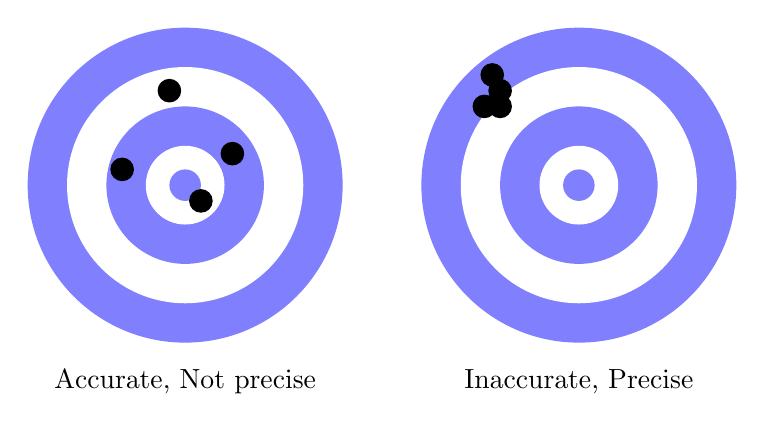
\begin{tikzpicture}
    % First target (High Accuracy, Low Precision)
    \begin{scope}
        \fill[blue!50] (0,0) circle (2);
        \fill[white] (0,0) circle (1.5);
        \fill[blue!50] (0,0) circle (1);
        \fill[white] (0,0) circle (0.5);
        \fill[blue!50] (0,0) circle (0.2);
        \fill (0.6,0.4) circle (0.15);
        \fill (-0.8,0.2) circle (0.15);
        \fill (0.2,-0.2) circle (0.15);
        \fill (-0.2,1.2) circle (0.15);
        \node at (0,-2.5) {Accurate, Not precise};
    \end{scope}
    \begin{scope}[xshift=5cm]
        \fill[blue!50] (0,0) circle (2);
        \fill[white] (0,0) circle (1.5);
        \fill[blue!50] (0,0) circle (1);
        \fill[white] (0,0) circle (0.5);
        \fill[blue!50] (0,0) circle (0.2);
        \fill (-1.2,1) circle (0.15);
        \fill (-1,1.2) circle (0.15);
        \fill (-1.1,1.4) circle (0.15);
        \fill (-1,1) circle (0.15);
        \node at (0,-2.5) {Inaccurate, Precise};
    \end{scope}
\end{tikzpicture}
\end{center}
\end{frame}

\begin{frame}{Summing up}
    \begin{itemize}
        \item Measuring a psychological construct requires four fundamental steps:
        \begin{enumerate}
            \item \textbf{Conceptual definition}: clarifying what is meant by the construct;
            \item \textbf{Operational definition}: translating the construct into something observable and measurable;
            \item \textbf{Implementation of the measure}: choosing or constructing the appropriate tool;
            \item \textbf{Evaluation of the measure}: testing the tool to verify its validity and reliability.
        \end{enumerate}
    \end{itemize}
\end{frame}

\begin{frame}{Summing up}
    \textbf{1. Conceptual definition}
    \begin{itemize}
        \item A clear definition of the construct is needed.
        \item Essential to consult the scientific literature.
    \end{itemize}
    \vspace{0.5em}
    \textbf{2. Operational definition}
    \begin{itemize}
        \item Specifies \emph{how} the construct will be measured.
        \item Multiple operational definitions possible for the same construct.
    \end{itemize}
\end{frame}

\begin{frame}{Summing up}
    \textbf{3. Implementing the measure}
    \begin{itemize}
        \item Use an existing tool: faster, already validated, comparable with other studies.
        \item Create a new measure: only if \emph{necessary}; pay attention to simplicity, clarity, and number of items.
    \end{itemize}
    \vspace{0.5em}
    \textbf{4. Evaluating the measure}
    \begin{itemize}
        \item Preliminary test with some participants.
        \item Verify: clarity of instructions, timing, comprehensibility.
        \item Gather feedback to correct any problems before data collection.
    \end{itemize}
\end{frame}

\section{Stata}
\begin{frame}{clear all ;)}
    \texttt{. webuse set data.califano.xyz} \\
    \texttt{. webuse masteristi}
\end{frame}

\end{document}
